% This is samplepaper.tex, a sample chapter demonstrating the
% LLNCS macro package for Springer Computer Science proceedings;
% Version 2.20 of 2017/10/04
%
\documentclass[runningheads]{llncs}
%
\usepackage{graphicx}
% Used for displaying a sample figure. If possible, figure files should
% be included in EPS format.
%
% If you use the hyperref package, please uncomment the following line
% to display URLs in blue roman font according to Springer's eBook style:
% \renewcommand\UrlFont{\color{blue}\rmfamily}

\begin{document}
%
\title{Comparison of Web Frameworks on Python and Node.js Platforms}
%
%\titlerunning{Abbreviated paper title}
% If the paper title is too long for the running head, you can set
% an abbreviated paper title here
%
\author{Ekaterina Eliseeva\orcidID{0000-0002-4616-6829} \and
Ilkhom Khafizov\orcidID{0000-0002-9340-5239} \and
Ilya Gosudarev\orcidID{0000-0003-4236-5991}}
%
\authorrunning{E. Eliseeva, I. Khafizov}
% First names are abbreviated in the running head.
% If there are more than two authors, 'et al.' is used.
%
\institute{ITMO University, Saint Petersburg, Russia}
%
\maketitle              % typeset the header of the contribution
%
\begin{abstract}
An important task when developing a server web application is to choose the right technological stack. The existence of a large number of Node.js and Python frameworks causes the problem of making the choice between them. This article compares the most popular frameworks by such criteria as code quality, support, performance. The first section explains the selection of frameworks for the study. The second section contains the results of the frameworks source code analysis. The third section compares framework performance based on test results. In conclusion, recommendations will be given on the choice of a framework based on the results of the comparison.

\keywords{web frameworks  \and Node.js \and Python \and web server \and framework performance }
\end{abstract}
%
%
%
\section{Introduction}
Nowadays, JavaScript and Python are the most popular programming languages. Python is a high-level general-purpose programming language that can be used in the development of all types of software, from simple automation scripting to system programming, game development and web applications ~\cite{ref_book1}. JavaScript is the only language that works on the client site. Node.js is an open-source JavaScript execution environment that allows to run JavaScript on the server side as well.

Web-based server frameworks make it easy to write, maintain and scale web applications. They provide tools and libraries that simplify common web development tasks, such as URL routing, database interaction, session support, and user authentication.

The performance of a web application directly depends on the right choice of technological stack, so the choice of language and infrastructure for the development of the server part of the application must be careful and thoughtful. The existence of a large number of Node.js and Python frameworks causes the problem of making the choice between them, especially for beginners. Therefore, it is necessary to conduct a comparative analysis of frameworks, to highlight important advantages and disadvantages.

\section{The choice of frameworks}
To compare Python and Node.js server frameworks, the frequency of frameworks usage on these platforms was analyzed (Fig.~\ref{fig1} and Fig.~\ref{fig2}) .


\begin{figure}
    \begin{center}
        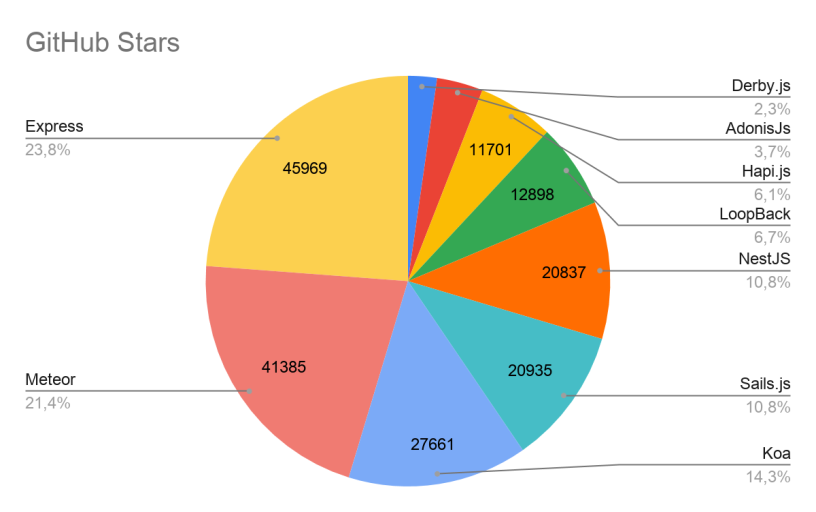
\includegraphics[width=0.7\textwidth]{fig-1.png}
    \end{center}
    \caption{GitHub Stars of Node.js frameworks.} \label{fig1}
\end{figure}

\begin{figure}
    \begin{center}
        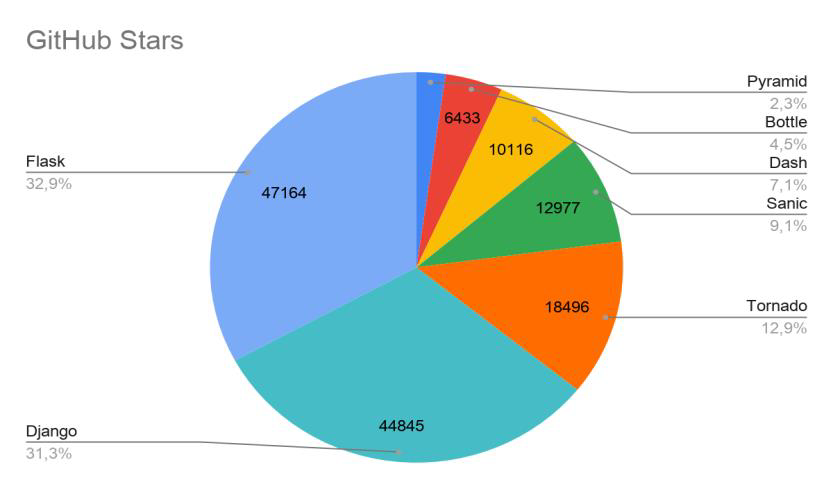
\includegraphics[width=0.7\textwidth]{fig-2.png}
    \end{center}
    \caption{GitHub Stars of Python frameworks.} \label{fig2}
\end{figure}
The most frequently used Express and Flask micro frameworks and Sails.js and Django frameworks using the MVC pattern were selected. Table ~\ref{tab1} shows GitHub Stars and the number of projects on GitHub that use Express, Sails.js, Flask and Django frameworks.


\begin{table}
\caption{Framework Rating on GitHub.}\label{tab1}
\begin{tabular}{|p{0.25\linewidth}|p{0.175\linewidth}|p{0.175\linewidth}|p{0.175\linewidth}|p{0.175\linewidth}|}
\cline{2-5}
\multicolumn{1}{l|}{} & Express  & Sails.js  & Flask    & Django   \\ 
\hline
GitHub Stars        & 45 919    & 20 922     & 47 164  & 44 845  \\ 
\hline
Used by             & 5 115 779 & 20 127 & 333 799   & 312 868     \\
\hline
\end{tabular}
\end{table}
%

From the diagrams and tables we can see that Express is the most popular among Node.js frameworks and the absolute leader in the number of uses in other repositories ~\cite{ref_url1}, Sails.js is one of the most frequently used Node.js MVC frameworks ~\cite{ref_url2}, Flask and Django are in the same degree ahead of other Python frameworks in terms of number of stars and use in other projects ~\cite{ref_url3}.


\section{Comparative analysis}
\subsection{Framework code analysis}
The following programs were used to analyze framework code:
\begin{itemize}
	\item SLOC \url{https://github.com/flosse/sloc} - to get the number of lines and comments in the framework code;
	\item complexity-report \url{https://github.com/escomplex/complexity-report} - to calculate Halstead's metrics, cyclomatic complexity, support index;
	\item Radon \url{https://pypi.org/project/radon} - to calculate the framework source code metrics on Python. 
\end{itemize}

Table ~\ref{tab2} shows the results of calculating the framework source code metrics.

\begin{table}
\caption{Framework source code analysis.}\label{tab2}
\begin{tabular}{|p{0.25\linewidth}|p{0.175\linewidth}|p{0.175\linewidth}|p{0.175\linewidth}|p{0.175\linewidth}|}
\hline
Metric &  Express  & Sails.js  & Flask    & Django\\
\hline
Number of lines of code & 13 013 & 203 936 & 10 486 & 271 045 \\
\hline
Number of comments & 5 635 & 106 244 & 4 255 & 58 742\\
\hline
Percentage of comments & 43.3\% & 52.1\% & 40.6\% & 21.7\%\\
\hline
Mean per-function Halstead effort & 2 345 & 2 475 & 510 & 2 324\\
\hline
Mean per-function cyclomatic complexity & 3.244 & 2.230 & 3.058 & 1.614\\
\hline
Maintainability index & 67 & 82 & 68.913 & 87.64\\
\hline
\end{tabular}
\end{table}

The highest percentage of code documentation has Sails.js; Express and Flask in this category also have good indicators. Express and Flask have high cyclomatic complexity, which makes their support more complex. Django doesn't have a lot of comments, but as well as Sails.js it has the lowest cyclomatic complexity and high support index, which means easier code support. 

Sails.js, Express and Flask have better documentation than Django, but their cyclomatic complexity is higher and the support index is lower, making their overall performance similar.


% -- subsection 3.2

\subsection{Performance analysis}

Framework performance tests were conducted on applications with the same functionality, with the following versions of the environment and frameworks:

\begin{itemize}
	\item Node v8.10.0, Express 4.17.1, Sails 1.2.3;
	\item Python 3.6.8, Flask 1.1.1, Django 2.2.6; 
\end{itemize}

The results of the performance study are also affected by the software and hardware used, which are as follows in this analysis:

\begin{itemize}
	\item Hardware: dual-core CPU Intel Core i5-3337U @ 1.80GHz, 6GB RAM;
	\item Software - Ubuntu operating system 18.04.3 LTS 64-bit; 
\end{itemize}
For the first test the application which returns a sequence of Fibonacci numbers for the parameter passed in URL has been created. The main performance indicators were identified as Requests per second, Time per request. These indicators were calculated using the Apache Benchmark web server testing tool \url{https://httpd.apache.org/docs/2.4/programs/ab.html} ~\cite{ref_url4}. 

Table ~\ref{tab3} shows the minimum processing time of a request, the time intervals for which 50\%, 75\% and 95\% of the requests were fulfilled, the number of requests per second and the average processing time of one request. A graph showing the number of completed requests to the server that returns a sequence of Fibonacci numbers for a certain time is shown in Figure ~\ref{fig3}.

\begin{table}
\caption{ Runtime and the number of requests to the server with Fibonacci.}\label{tab3}
\begin{tabular}{|p{0.15\linewidth}|p{0.1\linewidth}|p{0.1\linewidth}|p{0.1\linewidth}|p{0.1\linewidth}|p{0.2\linewidth}|p{0.2\linewidth}|}
\hline
& min, ms & 50\%, ms & 75\%, ms & 95\%, ms & Requests per second (mean) & Time per request (mean), ms\\
\hline
Express & 3 & 4 & 5 & 7 & 2019.35 & 4.952 \\
\hline
Sails.js & 11 & 14 & 16 & 23 & 638.40 & 15.664 \\
\hline
Flask & 8 & 18 & 21 & 26 & 524.58& 19.063 \\
\hline
Django & 13 & 38 & 43 & 50 & 263.66 & 37.928\\
\hline
\end{tabular}
\end{table}


\begin{figure}
    \centering
        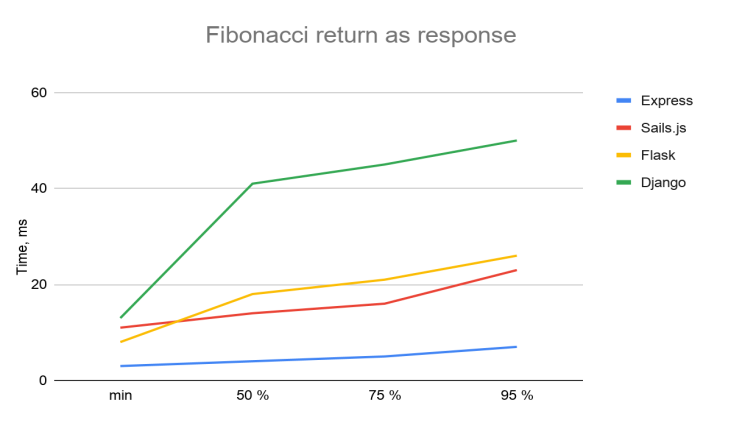
\includegraphics[width=0.7\textwidth]{fig-3.png}
    \caption{Fibonacci return as response.} \label{fig3}
\end{figure}

The Flask and Django frameworks have different implementations of working with JSON, therefore, the second test compares the performance of frameworks when working with JSON. The source data is an object that is converted to the ‘application / json’ format and returned as response. Table ~\ref{tab4}  and the graph in Figure ~\ref{fig4}  show the execution time of requests and the number of completed requests to the server returning JSON.


\begin{table}
\caption{ Runtime and the number of requests to the server sending JSON.}\label{tab4}
\begin{tabular}{|p{0.15\linewidth}|p{0.1\linewidth}|p{0.1\linewidth}|p{0.1\linewidth}|p{0.1\linewidth}|p{0.2\linewidth}|p{0.2\linewidth}|}
\hline
& min, ms & 50\%, ms & 75\%, ms & 95\%, ms & Requests per second (mean) & Time per request (mean), ms\\
\hline
Express & 4 & 5 & 6 & 9 & 1757.67 & 5.689 \\
\hline
Sails.js & 10 & 14 & 16 & 21 & 642.28 & 15.569 \\
\hline
Flask & 6 & 22 & 24 & 267 & 452.57 & 22.096 \\
\hline
Django & 5 & 34 & 37 & 43 & 293.35 & 34.089\\
\hline
\end{tabular}
\end{table}

\begin{figure}
    \centering
        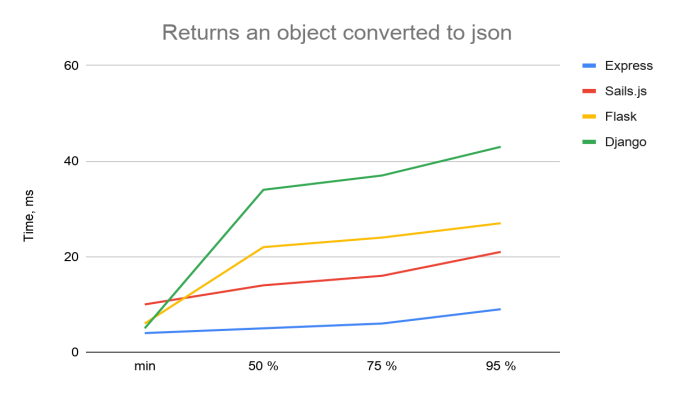
\includegraphics[width=0.7\textwidth]{fig-4.png}
    \caption{JSON returns as response.} \label{fig4}
\end{figure}

Express has the best performance indicators, the average number of processed requests which is more than twice as many as Sails.js. Flask also has good results, but is a little behind Sails.js. Django showed the slowest results according to the results of the analysis.

\section{Results}
The comparative analysis presented in this paper allows to make certain recommendations for choosing the right framework. According to the results of the frameworks source code analysis, Sails.js and Django have the best indicators. Performance tests have shown that the fastest framework is Express, in second place is Sails.js. Flask and Django frameworks are slower, but the average number of requests per second from Flask is almost twice as high as Django. 

So the problem of choice that has been put forward in the introduction can be solved according to the recommendations that follow. If a developer has programming experience in JavaScript, it is logical to choose one of the Node.js frameworks and avoid the time-consuming learning. Alternatively, the choice of Python may be more optimal because it is considered the most comprehensible and quickly learned language. For small projects it is better to choose Express or Flask, they allow to create a simple application and expand it if necessary. For larger projects the Sails.js or Django should be used, which allow to create a flexible, secure, scalable application by using built-in tools.
% ---- Bibliography ----
%
% BibTeX users should specify bibliography style 'splncs04'.
% References will then be sorted and formatted in the correct style.
%
% \bibliographystyle{splncs04}
% \bibliography{mybibliography}
%
\begin{thebibliography}{3}
\bibitem{ref_book1} 
Volobuev N.G. Sravnenie Web freimvorkov Python. Al'manah nauchnyh rabot molodyh uchenyh XLVI uchebnoj i nauchno-metodicheskoj konferencii Universiteta ITMO. Tom 4, 44-46.

\bibitem{ref_url1} 
Express vs Flask, \url{https://www.slant.co/versus/1277/1398/\textasciitilde{}express-js\_vs\_flask}. Last accessed 20 Oct 2019.

\bibitem{ref_url2} 
Sails.js vs Django, \url{https://www.slant.co/versus/1283/1746/\textasciitilde{}sails-js\_vs\_django}. Last accessed 20 Oct 2019.

\bibitem{ref_url3} 
Comparison Of Four Popular Node.js Frameworks, \url{https://www.toptal.com/nodejs/nodejs-frameworks-comparison}. Last accessed 22 Oct 2019.
\bibitem{ref_url4} 
Testirovanie proizvoditel'nosti web serverov. Apache Benchmark, \url{https://admins.su/site-speed-ab}. Last accessed 22 Oct 2019.

\end{thebibliography}
\end{document}
